\documentclass[a4paper,10pt]{article}
\usepackage[utf8]{inputenc}
\usepackage[brazil]{babel}
\usepackage{geometry}
\usepackage{enumitem}
\usepackage{titlesec}
\usepackage[hidelinks]{hyperref}
\usepackage{parskip}
\usepackage{graphicx}  % adicionar imagens
\geometry{margin=1in}
\titleformat{\section}{\large\bfseries}{}{0em}{}

\begin{document}

\begin{center}
    {\LARGE \textbf{Fernando Anselmo}} \\
    Brasília - DF, Brasil \\
    \href{mailto:fernando.anselmo74@gmail.com}{fernando.anselmo74@gmail.com} \\
    (61) 99874-0763 - 
    \href{https://www.linkedin.com/in/fernando-anselmo-bb423623/}{LinkedIn} \textbullet{}
    \href{https://github.com/fernandoans}{GitHub} \textbullet{}
    \href{https://www.youtube.com/channel/UC4VS4Emzy0TSbfgMfWcpnxA}{YouTube}
\end{center}

\section*{Resumo Profissional}
Líder técnico com atuação estratégica em projetos críticos de alta performance, além de forte envolvimento com docência e produção técnica. Autor de 18 livros e diversos artigos em revistas especializadas, além de palestrante em eventos da área de tecnologia. Busca constante por aprendizado e inovação, com o objetivo de gerar valor e promover melhorias contínuas nos processos de negócio. Especialista com foco em desenvolvimento e construção de diversos modelos arquiteturais. Experiência em modernização de sistemas legados, automação de pipelines CI/CD e integrações corporativas (AD, Protheus, Amadeus). 

\section*{Tecnologias e Ferramentas}
\vspace{8pt}
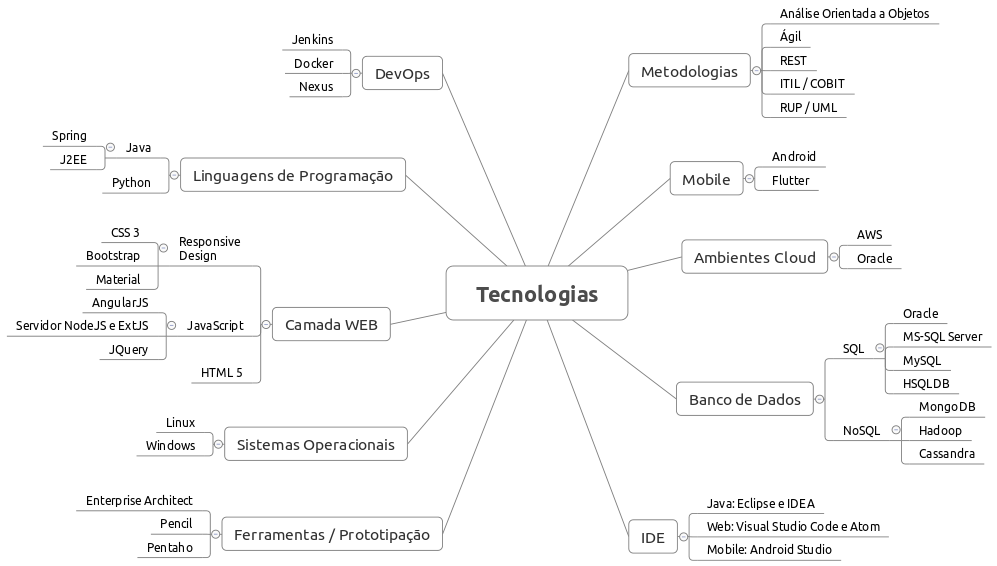
\includegraphics[width=0.9\textwidth]{imagens/tecnologias.png}

\section*{Experiência Profissional}

\textbf{Desenvolvedor FullStack Sênior – First Decision} \hfill Jan/2026 – Atual \\
Migrado para a First Decision para continuar as atividades no contrato do Ministério dos Transportes, desenvolvimento de projeto com Angular 17 e Java (Spring Boot com arquitetura Hexagonal - "Ports and Adapters"). Após a entrega do projeto fui alocado no Mauá/FalaBr para atuar com Experiência sólida com: Angular 21, Node.js e TypeScript com o uso de Inteligência Artificial. Neste projeto auxilio a equipe arquitetural em tarefas como: estruturação de ambientes com segregação de redes e controles de segurança; integração com bancos de dados relacionais (PostgreSQL, SQL Server, Oracle) e NoSQL; atuação em arquiteturas baseadas em microsserviços.

\textbf{Desenvolvedor FullStack Sênior – Qintess} \hfill Ago/2025 – Jan/2026 \\
Análise e desenvolvimento de sistemas para o cliente Ministério dos Transportes em tecnologia Java e Angular, atuar como Analista Full Stack para os sistemas, com modelo de Arquitetura Java/Hexagonal, também auxiliei em atividades como: definição de estratégias de versionamento e governança de código (Git); definição de ambientes; integração de aplicações via APIs REST. O contrato com a Qintess foi encerrado pelo Ministério.

\textbf{Desenvolvedor BackEnd Java – SEA Tecnologia} \hfill Nov/2024 – Mar/2025 \\
Contratado como Desenvolvedor Sênior Backend (Cooperado) para desenvolver tecnologias para o Liferay com Java. Alocado nos projeto PesqBrasil que realiza o cadastro de pescadores do Brasil, e em seguida no projeto do Portal do SESC. Neste período trabalhei com: implantação DevOps e DevSecOps; soluções de observabilidade; definição de estratégias de versionamento e governança de código (Git); definição de ambientes; integração de aplicações via APIs REST; desenho de soluções com alta disponibilidade, escalabilidade e contingência; planejamento de capacidade (capacity planning) e dimensionamento de ambientes. Após muito aprendizado entendo que é hora de olhar para o mercado, ter novos desafios, contribuir com toda minha bagagem em outra empresa.

\textbf{Analista de Sistemas IV – CNI/SESI} \hfill Nov/2021 – Out/2024 \\
Contratado pela CNI/SESI para atuar como Analista de Sistemas IV. Fui responsável pela refatoração de bases legadas em Java, com o objetivo de revitalizar e modernizar os projetos existentes. Atuei ativamente na construção de APIs para facilitar processos internos, incluindo a geração de relatórios com Jasper Reports e a autenticação de usuários via Active Directory (AD). Também trabalhei com plataformas Low Code, como Outsystems, Power Apps e Power Automate, desenvolvendo e mantendo diversas funcionalidades. Além disso, prestei suporte direto aos usuários, solucionando chamados com demandas variadas e contribuindo para a melhoria contínua dos serviços. Neste projeto também participei de tarefas como: definição e implantação de arquiteturas corporativas baseadas em containers (Kubernetes); estruturação e manutenção de pipelines CI/CD (GitLab CI e Jenkins); implantação de práticas DevOps e DevSecOps; implementação de soluções de observabilidade e integração de aplicações via APIs REST; desenho de soluções com alta disponibilidade, escalabilidade e contingência; planejamento de capacidade (capacity planning) e dimensionamento de ambientes. 

\textbf{Arquiteto de Soluções – Bancorbrás} \hfill Fev/2021 – Nov/2021 \\
Devido aos excelentes serviços prestados, foi contratado pela Bancorbrás para integrar o time de Arquitetura e definição de projetos utilizando tecnologias como Java com Spring Boot (Spring Data e Spring Batch), JBoss, Quarkus (com GraalVM e mensageria assíncrona) e testes unitários seguindo o padrão TDD. Participei da configuração de ambientes de integração contínua com Docker, Jenkins 2, SonarQube, Maven e Git. Possuo experiência prática com metodologias ágeis. Responsável por modernizar processos financeiros antigos implementados em Stored Procedures, convertendo-os para soluções modernas em Java com Spring Boot. Além disso, integrou sistemas como Protheus e Active Directory, otimizando os processos de Recursos Humanos. Neste projeto também trabalhei em soluções como: integração de aplicações via APIs REST; desenho de soluções com alta disponibilidade, escalabilidade e contingência; integração com bancos de dados relacionais e NoSQL; modelagem em arquiteturas baseadas em microsserviços.

\textbf{Desenvolvedor Backend – Mirante Tecnologia} \hfill Out/2019 – Fev/2021 \\
Contratado para atuar no desenvolvimento de projetos de software para o cliente Bancorbrás. Responsável pela construção de microsserviços corporativos utilizando o framework Spring Boot. Realizei a automação e disponibilização de serviços por meio da integração contínua com Jenkins e Docker. Atuei no desenvolvimento em Java, criação de testes unitários e implementação de pipelines de integração contínua. Possuo também experiência em ambientes de computação em nuvem, com destaque para a Oracle Cloud. Participei da configuração de ambientes de integração contínua com Docker, Jenkins 2, SonarQube, Maven e Git. Possuo experiência prática com metodologias ágeis. Responsável por modernizar processos financeiros antigos implementados em Stored Procedures, convertendo-os para soluções modernas em Java com Spring Boot. Além disso, integrou sistemas como Protheus e Active Directory, otimizando os processos de Recursos Humanos. Neste projeto também trabalhei em soluções como: integração de aplicações via APIs REST; desenho de soluções com alta disponibilidade, escalabilidade e contingência; integração com bancos de dados relacionais e NoSQL; modelagem em arquiteturas baseadas em microsserviços.

\section*{Experiência Profissional Docência}

\textbf{Professor de Informática} \hfill Fev/2023 – Atual \\
Contratado como professor no curso de Graduação em Tecnologia da Informação. Atuei inicialmente como substituto temporário durante o último semestre de 2022 e, ao término das turmas, fui convidado a integrar o corpo docente de forma permanente. Desde então, venho ministrando disciplinas e treinamentos nas áreas de Algoritmos, Técnicas de Programação Orientada a Objetos, Programação Mobile e Programação Web.

\textbf{Professor Pós e Graduação em Ciência de Dados} \hfill Ago/2018 – Atual \\
Contratado como professor nos cursos de Graduação e Pós-Graduação em Ciência de Dados. Leciono a disciplina de Introdução às Tecnologias de Ciência de Dados, aplicando metodologias ativas de ensino. A matéria abrange conteúdos como Python, bancos de dados Hadoop, pensamento analítico, qualidade de dados, mineração de dados, Big Data, além de introdução à robótica e automação. Minhas aulas focam em desenvolver competências práticas e analíticas, alinhadas às demandas do mercado de dados.

\textbf{Experiências Anteriores} \hfill Jan/1987 – Set/2019 \\
Lista completa de todas as minhas experiencias podem ser vistas no meu histórico do 
\href{https://www.linkedin.com/in/fernando-anselmo-bb423623/details/experience/}{LinkedIn}.

\section*{Formação Acadêmica}
\begin{itemize}[noitemsep]
  \item Pós-Graduação em Docência em Sistemas de Informações - Faculdade Iguaçu - Cursando
  \item Pós-Graduação em Arquitetura de Software - Faculdade Iguaçu - Cursando
  \item MBA em Gestão da Informação - Faculdade Iguaçu - Cursando
  \item MBA em Tecnologia para Negócios: Data Science e Big Data - Faculdade Iguaçu - Cursando
  \item Pós-Graduação em proficiência em tecnologias digitais para uma educação empreendedora - Secretaria de Educação GDF / SEBRAE - Cursando
  \item Pós-Graduação em Estatística Aplicada - Faculdade Anhanguera - 2020
  \item Técnico em Jogos Digitais - IFB - 2019
  \item Pós-Graduação em Gestão Empresarial Avançada - Faculdade JK - 2016
  \item Graduação em Gestão da Tecnologia da Informação - FacSenac - 2011
  \item Especialização em Programação - Faculdades Integradas da Católica - 1996
\end{itemize}

\section*{Certificações Relevantes}
\begin{itemize}[noitemsep]
  \item Java Champion - Oracle
  \item Certified AI Foundations Associate - Oracle
  \item Sun Certified Programmer Java 2 - Sun Microsystems
  \item Java SE 6 Programmer Certified - Oracle
  \item Java EE 5 Web Component Developer Certified - Oracle
  \item SCRUM Foundation - Diversas certificadoras
  \item Formação em Ciência de Dados - Cognitive Class
  \item Diversos Certificados de cursos que podem ser visualizados em \href{https://github.com/fernandoans/Certificados}{GitHub}
\end{itemize}

\section*{Idiomas}
\begin{itemize}[noitemsep]
  \item Inglês: Avançado
  \item Espanhol: Avançado (leitura e escrita)
\end{itemize}
\vspace{10pt} 
\section{MAIORES INFORMAÇÕES}
\begin{description}
	\item[Perfil no Linkedin] \url{http://www.linkedin.com/pub/fernando-anselmo/23/236/bb4}
	\item[GitHub] \url{https://github.com/fernandoans}
	\item[Canal no YouTube] \url{https://www.youtube.com/channel/UC4VS4Emzy0TSbfgMfWcpnxA}
	\item[Página Pessoal] \url{http://fernandoanselmo.orgfree.com/wordpress/}
	\item[Blog Pessoal] \url{http://fernandoanselmo.blogspot.com/}
\end{description}

\end{document}
